\documentclass[tikz,border=10pt]{standalone}
\usepackage{pgfplots}
\pgfplotsset{compat=1.18}
\usetikzlibrary{arrows.meta, positioning}

\begin{document}
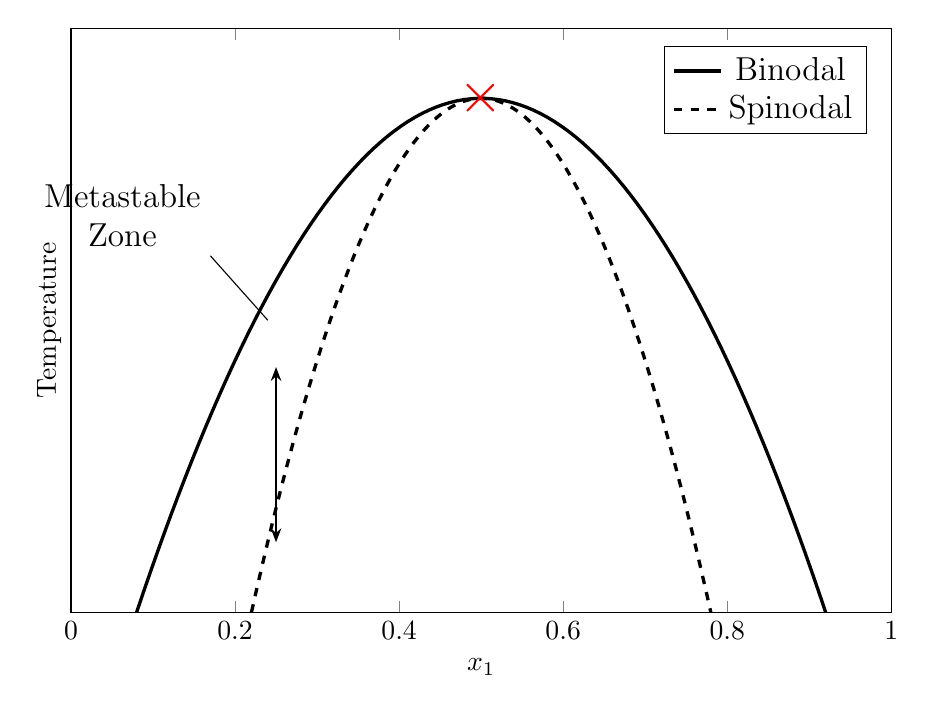
\begin{tikzpicture}
    \begin{axis}[
        % --- Axis Setup ---
        xlabel = {$x_1$},
        ylabel = {Temperature},
        xlabel style = {font=\large},
        ylabel style = {font=\large},
        % Domain and Range
        xmin = 0, xmax = 1,
        ymin = 0, ymax = 1,
        % Ticks
        xtick = {0.0, 0.2, 0.4, 0.6, 0.8, 1.0},
        ytick = \empty,
        % Styling
        axis lines = box,
        width = 12cm,
        height = 9cm,
        clip = false,
        % Legend
        legend pos = north east,
        legend style = {font=\large, draw=black}
    ]

        % Binodal curve (outer, solid)
        % y = -4.9887 * (x - 0.08) * (x - 0.92)
        \addplot[
            black,
            very thick,
            domain = 0.08:0.92,
            samples = 100
        ] {-4.9887*(x - 0.08)*(x - 0.92)};
        \addlegendentry{Binodal}

        % Spinodal curve (inner, dashed)
        % y = -11.2245 * (x - 0.22) * (x - 0.78)
        \addplot[
            black,
            very thick,
            dashed,
            domain = 0.22:0.78,
            samples = 100
        ] {-11.2245*(x - 0.22)*(x - 0.78)};
        \addlegendentry{Spinodal}

        % Critical point (red X) - make it more prominent
        \node[red, font=\huge, inner sep=0pt] at (axis cs:0.5, 0.88) {\textbf{$\times$}};

        % Metastable Zone annotation
        % Double-headed arrow between curves at x ~ 0.25
        % At x=0.25: binodal y ~ 0.455, spinodal y ~ 0.095
        \draw[{Stealth[length=5pt]}-{Stealth[length=5pt]}, thick]
            (axis cs:0.25, 0.12) -- (axis cs:0.25, 0.42);

        % Label with line pointing to arrow
        \node[anchor=east, font=\large, align=center] (metastable) at (axis cs:0.17, 0.68) {Metastable\\Zone};
        \draw[thin] (metastable.south east) -- (axis cs:0.24, 0.50);

    \end{axis}
\end{tikzpicture}
\end{document}
